\section{Einführung}
Wird Licht von Objekten gestreut, deren Ausdehnung in der Größenordnung der Wellenlänge liegt, so lässt sich die Lichtausbreitung nicht mehr wie in der geometrischen Objekt durch Strahlen beschreiben. Stattdessen führt der Wellencharakter des Lichtes zu einer Beugung und es entstehen Interferenzmuster.

Das Prinzip von Huygens-Fresnel besagt, das jeder Punkt auf einer Wellenfront als Ausgangspunkt einer Kugelwelle gesehen werden kann. Zu einem späteren Zeitpunkt lässt sich die Ausbreitung der Welle berechnen, indem man diese Elementarwellen überlagert.

\subsection{Frauenhofer-/Fernfeldbeugung}
In der Fernfeldbeugung wird angenommen, dass die einfallenden und die aufallenden Wellen nahezu eben sind. Dies ist eine gute Näherung, wenn die Lichtquelle weit vom Beugungselement und dieses weit vom Schirm entfernt ist.
\subsubsection{Beugung am Spalt}
Für einen Spalt mit Breite $b$ ergibt sich in einem Winkel $\theta$ zur optischen Achse die Intensität 

\begin{equation}
I(\vartheta)\propto b^2\left\{\frac{sin\beta}{\beta}\right\}^2
\label{spaltintens}
\end{equation}
\begin{figure}[!htb]
  \centering
  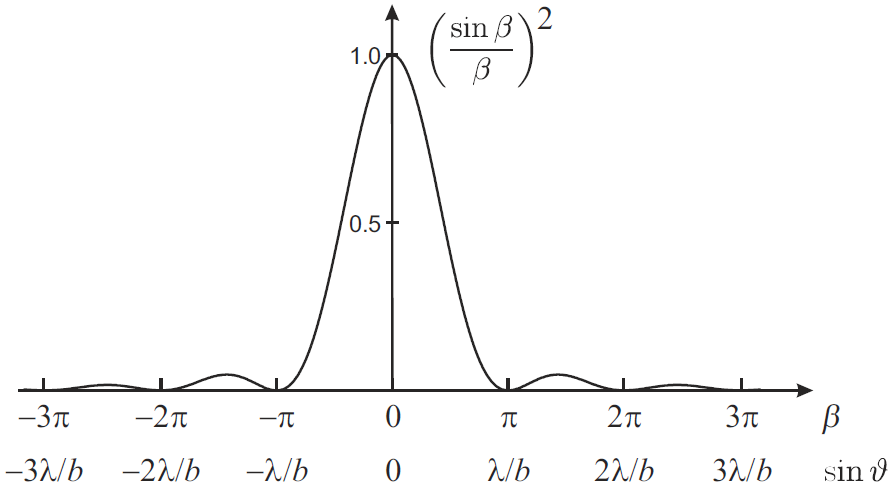
\includegraphics[width=.8\textwidth]{res/spaltintens}
  \caption{Lichtintensität hinter einem Beugungsspalt\footcite{anleitung-ss2015}}
  \label{fig:spaltintens}
\end{figure}
mit $\beta=(kb\sin\vartheta)/2=\pi\frac{b}{\lambda}\sin\vartheta$. Die Funktion $(\sin\beta/\beta)^2$ ist in \cref{fig:spaltintens} abgebildet. Sie hat für $\beta=0$ das Maximum 1 und Nullstellen für $\beta=\pm\pi, \pm 2\pi,\dots$. Auf einem in großem Abstand zum Spalt aufgestellten Schirm sind Minima zu sehen für Winkel $\vartheta$ mit 
\begin{equation}
\sin\vartheta=m\frac{\lambda}{b} \qquad\text{wobei}\qquad m=\pm1,\pm2,\dots
\label{eq:spaltmin}
\end{equation}
\subsubsection{Beugung am Gitter}
Ein Gitter besteht aus abwechselnd lichtdurch- bzw. undurchlässigen Sektoren. Die Gitterkonstante $g$ ist der Abstand zwischen benachbarten Streifen, $b$ die Breite eines Streifens und $N$ die Anzahl der Gitterlücken. Die Intensität bei einem Winkel $\vartheta$ zur optischen Achse beträgt dann
\begin{align}
I(\vartheta)&\propto \left[\frac{\sin(N\gamma)}{\sin\gamma}\right]^2\cdot\left[\frac{\sin\beta}{\beta}\right]^2 \qquad\text{mit}\nonumber \\
\gamma&=\pi\frac{g}{\lambda}\sin\vartheta \qquad \text{und}\qquad\beta=\pi\frac{b}{\lambda}\sin\vartheta=\frac{b}{g}\gamma
\label{eq:gitterintens}
\end{align}
\begin{figure}[!htb]
  \centering
  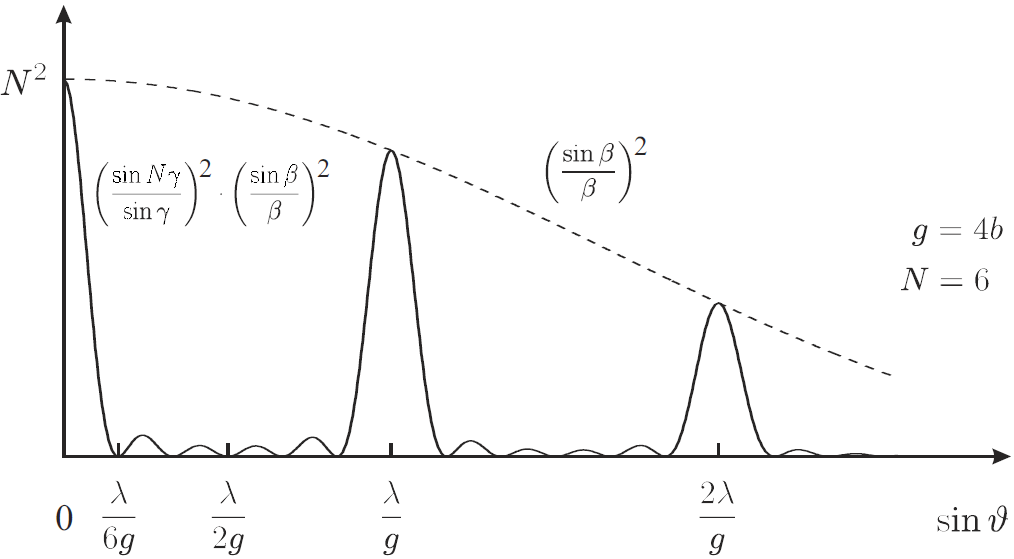
\includegraphics[width=.8\textwidth]{res/gitterintens}
  \caption{Lichtintensität hinter einem Gitter\footcite{anleitung-ss2015}}
  \label{fig:gitterintens}
\end{figure}
Die Maxima des Gitterfaktors $[\sin(N\gamma)/\sin\gamma]^2$ 
\begin{equation}
\sin\vartheta_m=m\frac{\lambda}{g} \qquad\text{mit}\quad m=0,\pm1,\pm2,\dots
\label{eq:gittermax}
\end{equation}

entsprechen Hauptmaxima auf dem Schirm. Hier gilt $[\sin(N\gamma)/\sin\gamma]^2=N^2$. Zwischen zwei Hauptmaxima liegen $N-1$ Minima bei 
\begin{equation}
\gamma=\pm\frac{\pi}{N},\pm\frac{2\pi}{N},\dots,\pm\frac{(N-1)\pi}{N},\pm\frac{(N+1)\pi}{N},\dots
\label{eq:gittermin}
\end{equation}
und $N-2$ Nebenmaxima ungefähr an den Punkten
\begin{equation}
\gamma=\pm\frac{3\pi}{2N},\pm\frac{5\pi}{2N},\dots\qquad .
\label{eq:gitternebenmin}
\end{equation}. 

Die Intensität $I_m$ des m-ten Hauptmaximums ist proportional zu 
\begin{equation}
I_m\propto \left[\frac{\sin(m\pi b/g)}{m\pi b/g}\right]^2
\label{eq:formfaktor}
\end{equation}. 
\refstepcounter{section}
\addcontentsline{toc}{section}{\protect\numberline{\thesection}Versuch}
\refstepcounter{subsection}
\addcontentsline{toc}{subsection}{\protect\numberline{\thesubsection}Versuchsaufbau}
\refstepcounter{subsection}
\addcontentsline{toc}{subsection}{\protect\numberline{\thesubsection}Kalibrierung des Wegaufnehmer}
\refstepcounter{subsection}
\addcontentsline{toc}{subsection}{\protect\numberline{\thesubsection}Einzelspalt}
\refstepcounter{subsection}
\addcontentsline{toc}{subsection}{\protect\numberline{\thesubsection}Doppel- und Einfachspalt}
\refstepcounter{subsection}
\addcontentsline{toc}{subsection}{\protect\numberline{\thesubsection}Doppelspalte}
\refstepcounter{subsection}
\addcontentsline{toc}{subsection}{\protect\numberline{\thesubsection}Mehrfachspalte}
\refstepcounter{subsection}
\addcontentsline{toc}{subsection}{\protect\numberline{\thesubsection}Vierfachspalt}
\section{Diskussion}
\subsection{Einzelspalt}
Hier wurde die unbekannte Wellenlänge $\lambda$ des Lasers mittels der Lage der Minima bestimmt. Da drei Werte von drei verschiedenen Spalten zur Verfügung standen, kann die Tauglichkeit dieser Methode an der Abweichung zwischen den Werten abgelesen werden. Die Differenz des größten und des kleinsten Wertes beträgt $\SI{765}{nm}-\SI{696}{nm}=\SI{69}{nm}$. Es handelte sich beim Versuch um einen roten Laser, was mit der berechneten Wellenlänge konsistent ist.
\subsection{Doppel- und Einfachspalt}
Aus \cref{eq:gitterintens} wird erwartet, dass die Intensitätsverteilung des Einfachspaltes eine Einhüllende der Intensitätsverteilung eines Doppelspaltes bildet. Dies ist in Abbildung 6 zu sehen. Zwischen dem nullten und dem ersten Hauptmaximum des Doppelspalts ist deutlich ein Nebenminimum erkennbar, was auch der Erwartung für ein Gitter mit $N=2$ entspricht. Allerdings fällt auf, dass die Intensität bei den Minima nicht auf 0 abfällt. Dies ist auf Licht von den Tischlampen und Streuung des Laserlichtes an den Wänden bzw. an der Luft zurückzuführen.
\subsection{Doppelspalte}
In Abbildung 6 ist zu sehen, dass die Spaltbreite sich auf die Breite der Einhüllenden auswirkt: Diese ist für $b=\SI{0.15}{mm}$ schmaler als für $b=\SI{0.10}{mm}$. Die Gitterkonstante scheint auf die Einhüllende keinen Einfluss zu haben, denn die Hauptmaxima der Messung für $g=\SI{0.25}{mm}$ berühren genau den Graphen für $g=\SI{1.0}{mm}$. Dies ist konsistent mit \cref{eq:gitterintens}, da im Formfaktor das Argument $\beta$ unabhängig von $g$ geschrieben werden kann.

Die Gitterkonstante beeinflusst den Abstand der Maxima zueinander: Für $g=\SI{1.0}{mm}$ liegen diese sichtbar näher als für $g=\SI{0.25}{mm}$. Auch dies ist konsistent mit \cref{eq:gitterintens}, da ein größerer Wert von $g$ zu einem größeren Faktor im Argument von $\sin\gamma$ im Nenner des Strukturterms führt, sodass sich die räumliche Frequenz der Maxima erhöht.
\subsection{Mehrfachspalte}
Die eingezeichneten Linien in Abbildung 7 entsprechen den aus der Wellenlänge berechneten Werte für die ersten beiden Hauptmaxima. Diese weichen leicht von den gemessenen Werten ab, allerdings ist dies noch im Rahmen des Fehlers, der sich aufgrund von Unsicherheit in der Wellenlänge fortpflanzt. Es wurde erwartet, dass die Intensität der Hauptmaxima mit $N^2$ steigt. Der Wert für $N=40$ ist nicht aussagekräftig, da der Laser nicht mehr als 5 Spalten ausgeleuchtet hat. Die anderen 3 Messwerte ensprechen der Erwartung, z.B. gilt für das 0te Hauptmaximum: Intensität für $N=3$: \num{41.3}, Intensität für $N=4$: \num{81.1}, und $\frac{41.3 \cdot 4^2}{81.1\cdot 3^2}=\num{0.91}\approx 1$.

Es wurde aus der Höhe des ersten Hauptmaximums der Wert $b/g=\num{0.611(120)}$ berechnet, was gut mit dem tatsächlichen Wert $b/g=\num{0.6}$ übereinstimmt. Dies bestätigt den Zusammenhang in \cref{eq:formfaktor}.

